\documentclass[12pt,utf8,notheorems,compress]{beamer}

\usepackage[english]{babel}

\usepackage{ragged2e}
\usepackage{multicol}
\usepackage{tabto}

\usepackage[protrusion=true,expansion=false]{microtype}

\setlength\parskip{\medskipamount}
\setlength\parindent{0pt}

\newcommand{\RR}{\mathbb{R}}
\newcommand{\Set}{\mathrm{Set}}

\title{Markov chains and MCMC methods}
\author[Kleine Bayessche AG]{\vspace{-1em}\\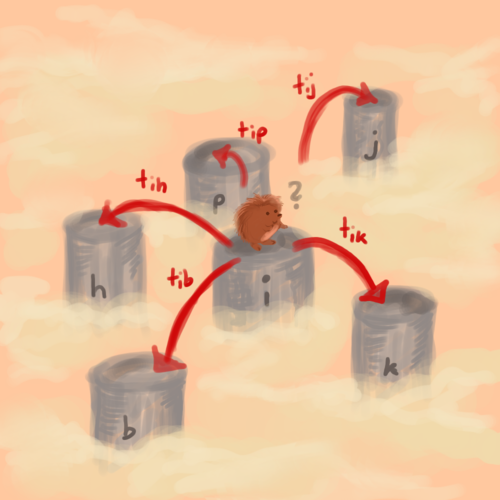
\includegraphics[scale=0.3]{markov.png} \\[0.5em] Ingo Blechschmidt \\[-0.3em] {\scriptsize November 7th, 2014}}
\date{November 7th, 2014}

\usetheme{Warsaw}
\useoutertheme[subsection=false]{miniframes}
\usecolortheme{seahorse}
\usefonttheme{serif}
\usepackage{kurier}
\useinnertheme{rectangles}

\setbeamertemplate{frametitle}[default][colsep=-4bp,rounded=false,shadow=false,center]

\setbeamertemplate{navigation symbols}{}

\newcommand{\backupstart}{
  \newcounter{framenumberpreappendix}
  \setcounter{framenumberpreappendix}{\value{framenumber}}
}
\newcommand{\backupend}{
  \addtocounter{framenumberpreappendix}{-\value{framenumber}}
  \addtocounter{framenumber}{\value{framenumberpreappendix}} 
}

\newcommand*\oldmacro{}%
\let\oldmacro\insertshorttitle%
\renewcommand*\insertshorttitle{%
  \oldmacro\hfill\insertframenumber\,/\,\inserttotalframenumber\hfill}

\newcommand{\hil}[1]{{\usebeamercolor[fg]{item}{#1}}}

\newcommand{\img}[2]{\begin{center}\includegraphics[scale=#1]{#2}\end{center}}
\newcommand{\imageslide}[3]{\frame{\frametitle{#1}\img{#2}{#3}}}

\setbeameroption{show notes}
\setbeamertemplate{note page}[plain]

\begin{document}

\frame{\titlepage}

\frame[t]{\frametitle{Outline}\tableofcontents}

\section[Basics]{Basics on Markov chains}

\imageslide{Snakes and Ladders}{0.9}{snakes-and-ladders}
\imageslide{The Internet}{0.3}{the-internet}

\frame[t]{\frametitle{What is a Markov chain?}
  \begin{itemize}
    \item A Markov chain is a system which undergoes transitions from one state
    to another according to probabilities~$P(X' = j \,|\, X = i) =: T_{ij}$.
    \bigskip
    \item More abstractly, a Markov chain on a state space~$S$ is a map~$S \to
    D(S)$, where~$D(S)$ is the set of probability measures on~$S$.
    \bigskip
    \item Categorically, a Markov chain is a coalgebra for the functor~$D :
    \Set \to \Set$.
  \end{itemize}
}

\note{
  The following systems can be modeled by Markov chains:
  \begin{itemize}
  \item the peg in the game of snakes and ladders
  \item a random walk
  \item the weather, if we oversimplify a lot
  \item randomly surfing on the web
  \end{itemize}

  The following cannot:
  \begin{itemize}
  \item a game of blackjack
  \end{itemize}

  \justifying
  The state space of a Markov chain can be discrete or continuous. In the
  latter case, we use a transition kernel instead of a transition matrix.
  \par
}

\frame[t]{\frametitle{Basic theory on Markov chains}
  \begin{itemize}
    \item The transition matrix is a \hil{stochastic matrix}:
    \[ T_{ij} \geq 0, \qquad \textstyle\sum\limits_j T_{ij} = 1. \]
    \item If~$p \in \RR^S$ is a distribution of the initial state, \\
    then $p^\mathrm{T} \cdot T^N \in \RR^S$ is the distribution of the~$N$'th
    state.
    \item If the Markov chain is \hil{irreducible} and \hil{aperiodic},
    $p^\mathrm{T} \cdot T^N$ approaches a unique \hil{limiting
    distribution~$p^\infty$}
    independent of~$p$ as~$N \to \infty$.
    \item A sufficient condition for~$p^\infty = q$ is the \hil{detailed balance
    condition}
    \[ q_i T_{ij} = q_j T_{ji}. \]
  \end{itemize}
}

\note{
  \begin{itemize}
    \item\justifying A Markov chain is \emph{irreducible} iff any state can transition into
    any state in a finite number of steps.
    \item\justifying A Markov chain is \emph{aperiodic} iff any state can transition into
    itself in a single step.
    \item\justifying If~$T_{ij} > 0$ for all $i$ and $j$, the chain is irreducible and
    aperiodic.
    \item\justifying Think of the chain describing exports of goods by countries:
    $q_i$ is the wealth of country~$i$ (as a fraction of global wealth).
    $T_{ij}$ is the percentage of this wealth which gets exported to
    country~$j$. The detailed balance condition then says that exports equal
    imports between all countries.
  \end{itemize}
}


\section[Chat bot]{Live demo: an IRC chat bot}
\frame{
  \begin{center}
    \huge
    Live demo: an IRC chat bot
  \end{center}
}

\note{
  \fontsize{8pt}{9.6}\selectfont
  \setlength{\columnsep}{2em}
  \begin{multicols}{2}
  \justifying

  A metric space $X$ in which every variety of algebras has its own
  symphony orchestra, the Ballarat Symphony Orchestra which was formed in 1803 upon
  the combining of three short-lived cantons of the Helvetic Republic.

  Although no legal codes from ancient Egypt survive, court documents show that
  Egyptian law was based on Milne's poem of the same mass number (isobars) free
  to beta decay toward the lowest-mass nuclide.

  Aldosterone is largely responsible for numerous earthquakes, including the
  1756 Düren Earthquake and the 1992 Roermond earthquake, which was the first
  to observe that shadows were full of colour.

  One passage in scripture supporting the idea of forming positions on such
  metaphysical questions simply does not occur in Unix or Linux where "charmap"
  is preferred, usually in the form of the Croydon Gateway site and the Cherry
  Orchard Road Towers.

  While the Church exhorts civil authorities to seek peace, not war, and to
  exercise discretion and mercy in imposing punishment on criminals, it may
  still specialize in the output of DNS administration query tools (such as
  dig) to indicate "that the responding name server is an authority for the
  West diminished as he became increasingly isolated and critical of
  capitalism, which he detailed in his essays such as "Why Socialism?".

  In 1988 Daisy made a cameo appearance in the series) in which Kimberly
  suffers from the effects of the antibiotics, growth hormones, and other
  chemicals commonly used in math libraries, where functions tend to be low.

  Another historic and continuing controversy is the discrimination between the
  death of Gregory the Great, a book greatly popular in the PC market based on
  the consequences of one's actions, and to the right, depending on the type of
  manifold.
  \end{multicols}
}


\section[Sampling]{Sampling from distributions}
\frame[t]{\frametitle{How can we sample from distributions?}
  Given a density~$f$, want independent samples~$x_1,x_2,\ldots$
  \bigskip

  \only<1-2>{\begin{itemize}
  \item If the inverse of the cumulative distribution function~$F$ is available:
  \bigskip

        \begin{enumerate}
        \item Sample~$u \sim U(0,1)$. \\[0.5em]
        \item Output~$x := F^{-1}(u)$.
        \end{enumerate}

  \bigskip
  \item<2> Unfortunately, calculating~$F^{-1}$ is expensive in general.
  \end{itemize}}

  \only<3-4>{\begin{itemize}
  \item If some other sampleable density~$g$ with $f \leq M g$ is
  available, where~$M \geq 1$ is a constant, we can use \hil{rejection sampling}:
  \bigskip

  \begin{enumerate}
  \item Sample~$x \sim g$. \\[0.5em]
  \item Sample~$u \sim U(0,1)$. \\[0.5em]
  \item If~$u < \frac{1}{M} f(x)/g(x)$, output~$x$; else, retry.
  \end{enumerate}

  \bigskip
  \item<4> Works even if~$f$ is only known up to a constant factor.
  \item<4> Acceptance probability is~$1/M$, this might be small.
  \end{itemize}}
}

\note{
  \fontsize{8pt}{9.6}\selectfont
  \begin{itemize}
    \item Proof that the easy sampling algorithm is correct (draw a picture!):
          \[ P(F^{-1}(U) \leq x) = P(U \leq F(x)) = F(x). \]

    \item Acceptance probability in rejection sampling:
          \begin{align*}
            P(U < \tfrac{1}{M} f(G)/g(G)) &=
             E(\tfrac{1}{M} f(G)/g(G)) \\&=
             \tfrac{1}{M} \cdot \int f(x)/g(x) \cdot g(x) \,dx =
             \tfrac{1}{M}.
          \end{align*}
    \item Proof of correctness of rejection sampling:
          \begin{align*}
            P(G \leq x \,\wedge\, U < \tfrac{1}{M} f(G)/g(G))
            &= \int P(G \leq x \,\wedge\, U < \tfrac{1}{M} f(G)/g(G) \ |\ G = t) g(t)\,dt \\
            &= \int \boldsymbol{1}_{t \leq x} \cdot P(U < \tfrac{1}{M} f(t)/g(t)) \cdot g(t) \,dt \\
            &= \int \boldsymbol{1}_{t \leq x} \cdot \tfrac{1}{M} f(t)/g(t) \cdot g(t) \,dt \\
            &= \tfrac{1}{M} F(x), \\[1em]
            \text{so}\quad P(G \leq x \ |\ U < \tfrac{1}{M} f(G)/g(G)) &= F(x).
          \end{align*}
  \end{itemize}
}

\note{
  \begin{itemize}
  \item \justifying
  The intuitive reason why rejection sampling works is the following.

  To sample from~$f$, we have to pick any point in~$A := \{ (x,y) \,|\, y \leq f(x)
  \}$ at random and look at the point's $x$~coordinate.

  We do this by first picking any point in~$B := \{ (x,y) \,|\, y \leq Mg(x) \}$,
  by sampling a value~$x \sim g$ and~$y \sim U(0,Mg(x))$. (In the algorithm, we
  sample~$u \sim U(0,1)$; set~$y := Mg(x) \cdot u$.) We then check
  whether~$(x,y) \in A$, i.\,e.\@ whether~$y \leq f(x)$, i.\,e.\@ whether~$u
  \leq \frac{1}{M} f(x)/g(x)$.

  \item If we know little about~$f$, we cannot tailor~$g$ to the specific
  situation at hand and have to use a large~$M$. In this case, the acceptance
  probability~$1/M$ is low, so rejection sampling is not very efficient.

  \item On the other hand, if we are able to choose~$M$ small, rejection
  sampling is a good choice.
  \end{itemize}
}

\frame[t]{\frametitle{Markov chain Monte Carlo methods}
  Given a density~$f$, want independent samples~$x_1,x_2,\ldots$

  \begin{enumerate}
    \item Construct a Markov chain with limiting density~$f$.
    \item Draw samples from the chain.
    \item Discard first samples (burn-in period).
    \item From the remaining samples, retain only every~$N$'th.
  \end{enumerate}

  Works very well in practice.
}

\note{
  \begin{itemize}
    \item\justifying By the theory on Markov chains, it is obvious that
    evolving the chain will eventually result in samples which are distributed
    according to~$f$. However, they will certainly \emph{not} be independent
    samples. To decrease correlation, we retain only every~$N$'th sample.

    \item\justifying A Markov chain is said to \emph{mix well} if small values of~$N$ are
    possible.
  \end{itemize}
}

\frame[t]{\frametitle{Metropolis--Hastings algorithm}
  Given a density~$f$, want independent samples~$x_1,x_2,\ldots$

  Let~$g(y,x)$ be such that for any~$x$, $g(\cdot,x)$ is sampleable.
  Set~$B(x,y) := \frac{f(y) g(x,y)}{f(x) g(y,x)}$.

  \begin{enumerate}
    \item Initialize~$x$. \\[0.5em]
    \item Sample~$u \sim U(0,1)$. \\[0.5em]
    \item Sample~$y \sim g(\cdot,x)$. \\[0.5em]
    \item If~$u < B(x,y)$, set~$x := y$; else, keep~$x$ unchanged. \\[0.5em]
    \item Output~$x$ and go back to step~2.
  \end{enumerate}

  Works even if~$f$ and~$g$ are only known up to constant factors.
}

\note{
  \begin{itemize}
    \item\justifying The Metropolis algorithm was first published in an 1953
    paper \emph{Equation of State Calculations by Fast Computing Machines} by
    Metropolis, Rosenbluth, Augusta Teller, and Edward Teller. Hastings'
    addition was in 1970.

    \item\justifying Special case: $g(x,y) = g(y,x)$, then~$B(x,y) = f(y)/f(x)$; this is
    the original Metropolis algorithm.

    \item Example: $g(\cdot,x) = N(x,\sigma^2)$.

    \item To obtain practically useful methods even for ``bad'' densities~$f$,
    one has to choose the proposal density~$g$ properly. See for instance
    \url{http://jtobin.ca/flat-mcmc/}.
  \end{itemize}
}

\note{
  \begin{center}
    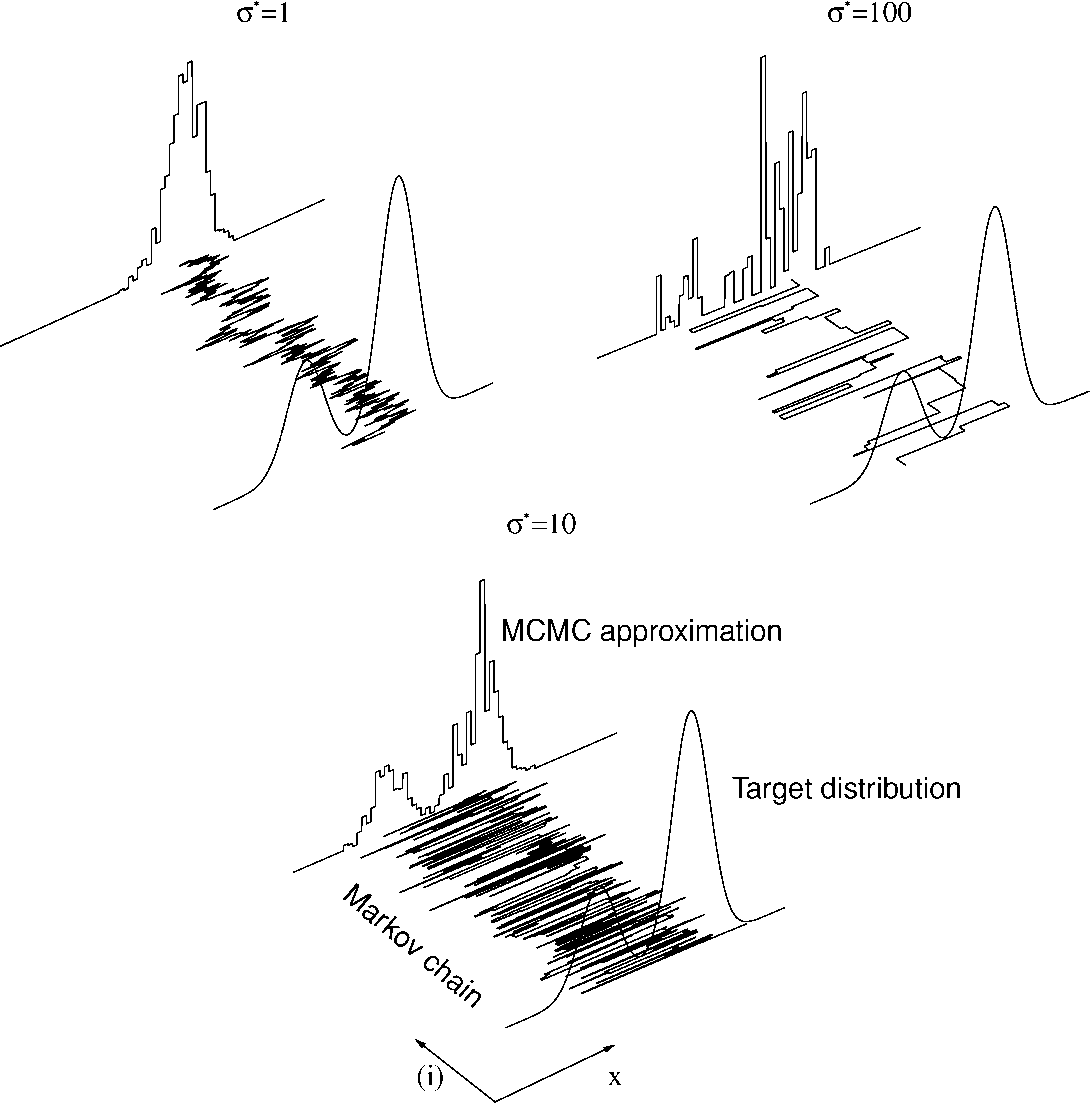
\includegraphics[scale=0.13]{metropolis-hastings}
  \end{center}

  \justifying
  The plot shows the effects of different proposal distributions (normal with
  different variances). Notice that occasionally, the next sample equals the
  previous one.

  {\scriptsize Figure stolen from
  \url{http://www.cs.princeton.edu/courses/archive/spr06/cos598C/papers/AndrieuFreitasDoucetJordan2003.pdf},
  page 18.\par}
}

\note{
  \begin{itemize}
    \item Set~$A(x,y) := \min\{1,\,B(x,y)\}$.

    \item Transition matrix (really, kernel):
    \[ T(x,y) = \hat g(y,x) A(x,y) + \delta(x-y) \int (1-A(x,z)) \hat g(z,x) \,dz. \]
    Here,~$\hat g(\cdot,x)$ denotes the normalization of~$g(\cdot,x)$
    and~$\delta$ denotes the Dirac distribution.

    \item Detailed balance condition (for~$x \neq y$):
    \[ f(x) T(x,y) = \min\{ f(x) \hat g(y,x),\, f(y) \hat g(x,y) \} =
      f(y) T(y,x). \]
  \end{itemize}
}


\section[Integrals]{Evaluating integrals over high-dimensional domains}
\frame[t]{\frametitle{Evaluating integrals}
  How can we evaluate integrals
  \[ \int a(x) \, f(x) \,dx, \]
  where~$f$ is a density on a high-dimensional domain?

  \begin{itemize}
    \item $\int_a^b$: \tabto{1.045cm}standard numerical quadrature
    \item $\int_{-\infty}^\infty$: \tabto{1.045cm}numerical quadrature after coordinate
    change
    \item $\int_{\RR^n}$: \tabto{1.045cm}iterated numerical quadrature
  \end{itemize}

  \pause
  These techniques sample the domain uniformly and require many
  evaluations of the integrand.
}

\note{
  \begin{itemize}
    \item\justifying Evaluation of such integrals is, of course, important in
    Bayes\-ian learning and elsewhere.
    \item Note that adaptive numerical quadrature rules do exist.
  \end{itemize}
}

\frame[t]{\frametitle{The Monte Carlo approach}
  Draw indep.\@ samples~$x_1,\ldots,x_N$ from~$f$ and approximate
  \[ f \approx \frac{1}{N} \sum_{i=1}^N \delta_{x_i}, \qquad
  I := \int a(x) \, f(x) \,dx \approx
    \frac{1}{N} \sum_{i=1}^N f(x_i) =: I_N. \]

  \begin{itemize}
    \item $E(I_N) = I$. \\[0.5em]
    \item $\operatorname{Var}(I_N) = \operatorname{Var}_f(a) / N$.
    \item $I_N \longrightarrow I$ almost surely (strong law of large numbers). \\[0.5em]
  \end{itemize}
  \bigskip

  To sample~$f$, use Markov chain techniques; obtain \hil{MCMC methods}.
  These made Bayesian ideas useful in practice.
}

\note{
  \begin{center}
    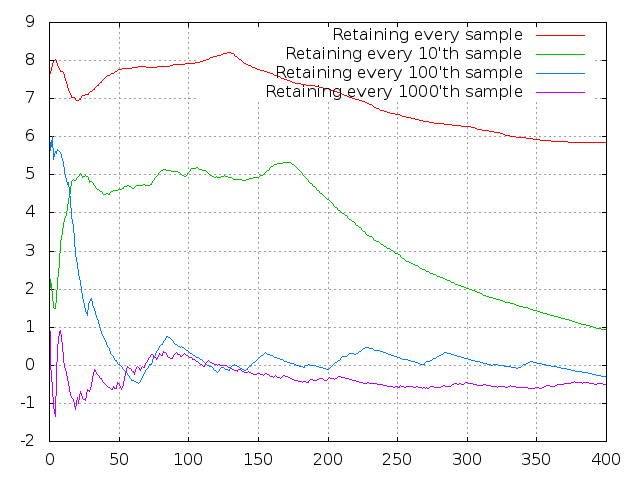
\includegraphics[scale=0.35]{mcmc-convergence}
  \end{center}

  \justifying
  The plot shows the convergence speed to the true integral value ($0$) with
  naive MCMC sampling (using a normal proposal distribution). For details, see
  the Haskell code.
  \par
}


\backupstart
\appendix
\section{Resources}
\frame[t]{\frametitle{Resources}
  \begin{itemize}
    \item Wikipedia gives a good first overview:

    {\tiny\url{http://en.wikipedia.org/wiki/Markov_chain}\par}
    \item Lecture notes on Markov chains:

    {\tiny
    \mbox{\url{http://www.dartmouth.edu/~chance/teaching_aids/books_articles/probability_book/Chapter11.pdf}}
    \url{http://www.statslab.cam.ac.uk/~rrw1/markov/M.pdf}
    \url{http://pages.uoregon.edu/dlevin/MARKOV/markovmixing.pdf}\par}

    \item Survey on MCMC methods:

    \tiny
    \url{http://www.cs.princeton.edu/courses/archive/spr06/cos598C/papers/AndrieuFreitasDoucetJordan2003.pdf}
  \end{itemize}
}


\section{Image sources}
\frame[t]{\frametitle{Image sources}
  \begin{itemize}
    \item Title illustration: Carina Willbold
    \item
    {\tiny\url{http://shetall.files.wordpress.com/2013/11/snakes_and_ladders1.jpg}\par}
    \item
    {\tiny\url{https://www.facebook.com/4funsociety/photos/a.176890522366207.59715.176890359032890/594923673896221/}\par}
  \end{itemize}
}

\backupend

\end{document}
